\section{Empirical Validation of the Minimum Displacement Assumption}
\label{app:displacement}

This section provides empirical support for~\cref{asm:edit} by measuring the activation displacement induced by five unlearning methods and verifying that the displacement propagates to semantic neighbors in proportion to their overlap with the target concept.

\paragraph{Setup.}
We extract cross-attention activations at \texttt{mid\_block.attentions.0} at step $t^*{=}25$ of 50 DDIM steps from five unlearning methods applied to erase \texttt{horse}: ESD, EDiff, SalUn, AdvUnlearn, and STEREO. For each method, we compare activations between the original model $\mathcal{D}_\theta$ and the concept-erased model $\mathcal{D}_{\hat\theta}$ under matched random seeds, so that observed differences reflect the unlearning edit rather than sampling variance. We measure mean displacement $\|\Phi_{\hat\theta}(p) - \Phi_\theta(p)\|_2$ across three prompt categories:
\begin{itemize}
    \item \emph{Target} prompts containing the erased concept (\texttt{horse});
    \item \emph{Neighbor} prompts containing semantically related concepts (\texttt{pony}, \texttt{donkey}, \texttt{deer});
    \item \emph{Control} prompts containing semantically isolated concepts (\texttt{castle}, \texttt{car}).
\end{itemize}
% For each prompt category, we use the same 50 shared templates as in~\cref{app:activation_regions}, differing only in the concept word. And~\cref{fig:displacement} reports the mean displacement by method and prompt category. Two patterns emerge.
For each prompt category, we use the same 50 shared templates as in~\cref{app:activation_regions}, differing only in the concept word. Activations are mean-pooled across spatial and token dimensions to produce a single vector per prompt, so the absolute magnitudes reported here are token-averaged and not directly comparable to the unpooled, full-tensor displacement values reported at a different layer in~\cref{app:displacement_kappa} (\cref{tab:displacement}); the two appendices probe different facets of the propagation mechanism --- this one establishes the \emph{ordering} $\Delta_{\mathrm{target}}, \Delta_{\mathrm{neighbor}} > \Delta_{\mathrm{control}}$ within a single target, while~\cref{app:displacement_kappa} establishes the \emph{$\hat\kappa$-scaling} of $\Delta_{\mathrm{neighbor}}$ across targets. \Cref{fig:displacement} reports the mean displacement by method and prompt category. Two patterns emerge.

First, all five methods produce substantial target displacement ($\Delta_{\mathrm{target}} \in [6.0, 9.9]$), confirming that $\varepsilon$-robust erasure requires non-trivial activation displacement as posited by~\cref{asm:edit}. Absolute target magnitudes vary across methods, reflecting different unlearning strategies and intervention layers; it is worth mentioning that these magnitudes are not comparable measures, as different methods operate on different subspaces.

Second, the displacement propagates to semantic neighbors: for every method, $\Delta_{\mathrm{neighbor}} \geq \Delta_{\mathrm{control}}$ with the gap ranging from $0.9$ (SalUn) to $6.9$ (STEREO). This gap is the empirical signature of the propagation mechanism in~\cref{thm:tradeoff}: displacement within $\mathcal{R}_{c_u}$ leaks into overlapping neighbor regions in proportion to $\kappa$, causing greater collateral displacement for high-$\kappa$ neighbors than for low-$\kappa$ controls. EraseDiff exhibits the smallest cross-category variation, suggesting it operates in a low-selectivity regime where $\kappa$-modulated propagation falls below our measurement granularity.

Third, STEREO is the only method for which $\Delta_{\mathrm{neighbor}} > \Delta_{\mathrm{target}}$, while simultaneously achieving the lowest control displacement ($2.1$). This produces a propagation gap of $6.9$, more than $2.7\times$ larger than any other method. This pattern is consistent with our analysis of STEREO in~\cref{rem:stereo}: by suppressing the entire subspace spanned by the adversarial tokens $v_1^*, v_2^*$ rather than the target alone, STEREO displaces neighbor concepts that lie within this shared subspace by even more than the target itself, while leaving semantically isolated concepts largely intact. 

These measurements support two claims central to our analysis. The uniform presence of nontrivial target displacement validates the precondition of~\cref{asm:edit}. The systematic neighbor, control gap, and STEREO's amplified version of it, validate the propagation claim in Step~2 of the proof: methods are not merely displacing the target in isolation but are displacing overlapping regions of activation space, with the magnitude of this collateral displacement modulated by the geometric overlap $\kappa$ predicted by~\cref{thm:tradeoff}. The robust prediction of the theorem is the \emph{ordering} $\Delta_{\mathrm{neighbor}} > \Delta_{\mathrm{control}}$ within each method and its scaling with $\kappa$ across concept types, not specific numerical values.


\begin{figure}[t]
\centering
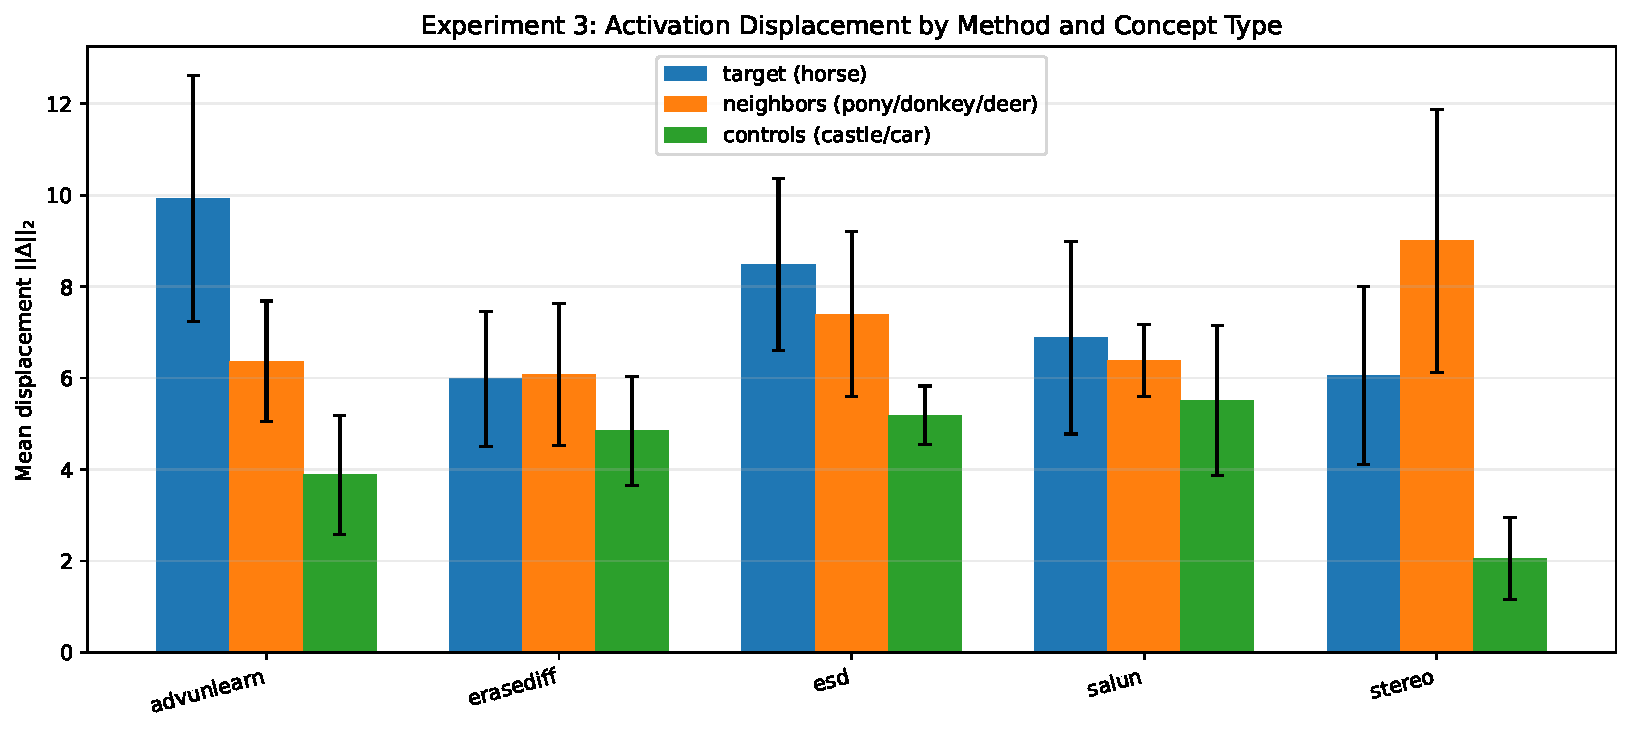
\includegraphics[width=\linewidth]{img/fig_displacement_by_method.pdf}
\caption{
Mean activation displacement $\|\boldsymbol{\Phi}_{\hat\theta}(p) - \boldsymbol{\Phi}_\theta(p)\|_2$ for five unlearning methods erasing \texttt{horse}. Target prompts (blue) confirm~\cref{asm:edit}: erasure requires measurable displacement. Neighbor prompts (orange) are displaced more than control prompts (green) for all methods, consistent with the propagation mechanism in~\cref{thm:tradeoff}.
}
\label{fig:displacement}
\end{figure}
\begin{comment}
    \paragraph{Empirical validation.}
To verify that unlearning methods produce measurable activation displacement, we extract cross-attention activations at \texttt{mid\_block.attentions.0}
(step 25/50) from five unlearning methods applied to erase \texttt{horse},
using matched random seeds between the original and unlearned models. Figure~\ref{fig:displacement} reports the mean displacement across three prompt categories:
target (\texttt{horse}), neighbors (\texttt{pony}, \texttt{donkey}, \texttt{deer}),
and controls (\texttt{castle}, \texttt{car}).
\begin{figure}[t]
\centering
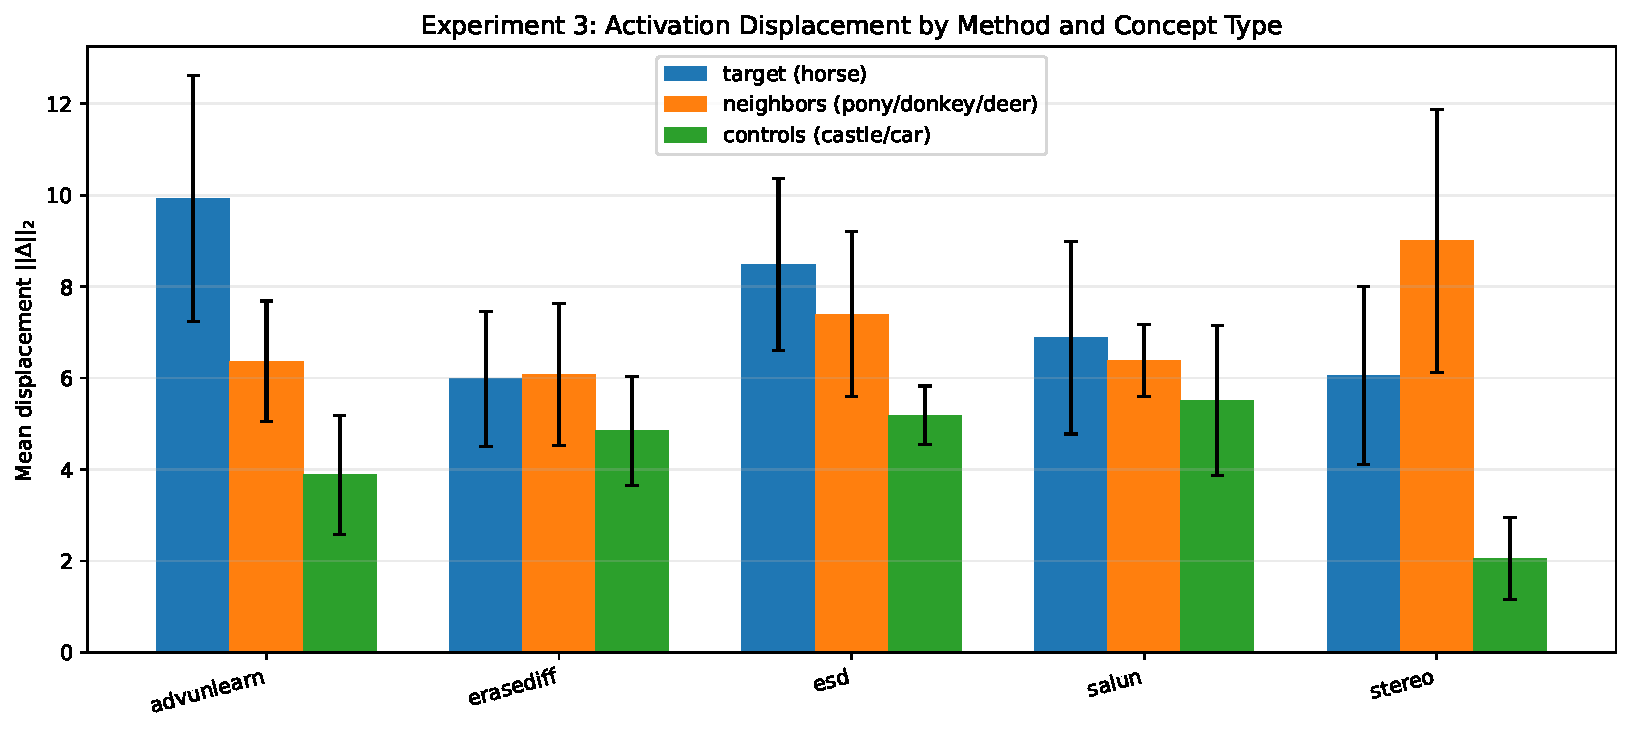
\includegraphics[width=\linewidth]{img/fig_displacement_by_method.pdf}
\caption{
Mean activation displacement $\|\Phi_{\hat\theta}(p) - \Phi_\theta(p)\|_2$
for five unlearning methods erasing \texttt{horse}.
Target prompts (blue) confirm Assumption~\ref{asm:edit}:
erasure requires measurable displacement.
Neighbor prompts (orange) are displaced more than control prompts (green)
for all methods, with the largest gap for STEREO ($3.26$),
consistent with the propagation mechanism in Theorem~\ref{thm:tradeoff}.
\ali{it might be better if the gap that you mention in the caption are better presented in the figure. just looking at the figure shows a different conclusion (i.e., there are other methods that displace neighbors more than STEREO}
}
\label{fig:displacement}
\end{figure}
\end{comment}